\section{Self Study 4: Refinement, normalization, and SQL-DDL}
\deadline{24}{3}{2014}
This document is formatted as closely as possible to the list of requirements for the report in the self study 4 exercises.

\subsection{Revised ER diagram}
We have merely added Chen and [min,max] notation.

\begin{figure}[h]
  \centering
  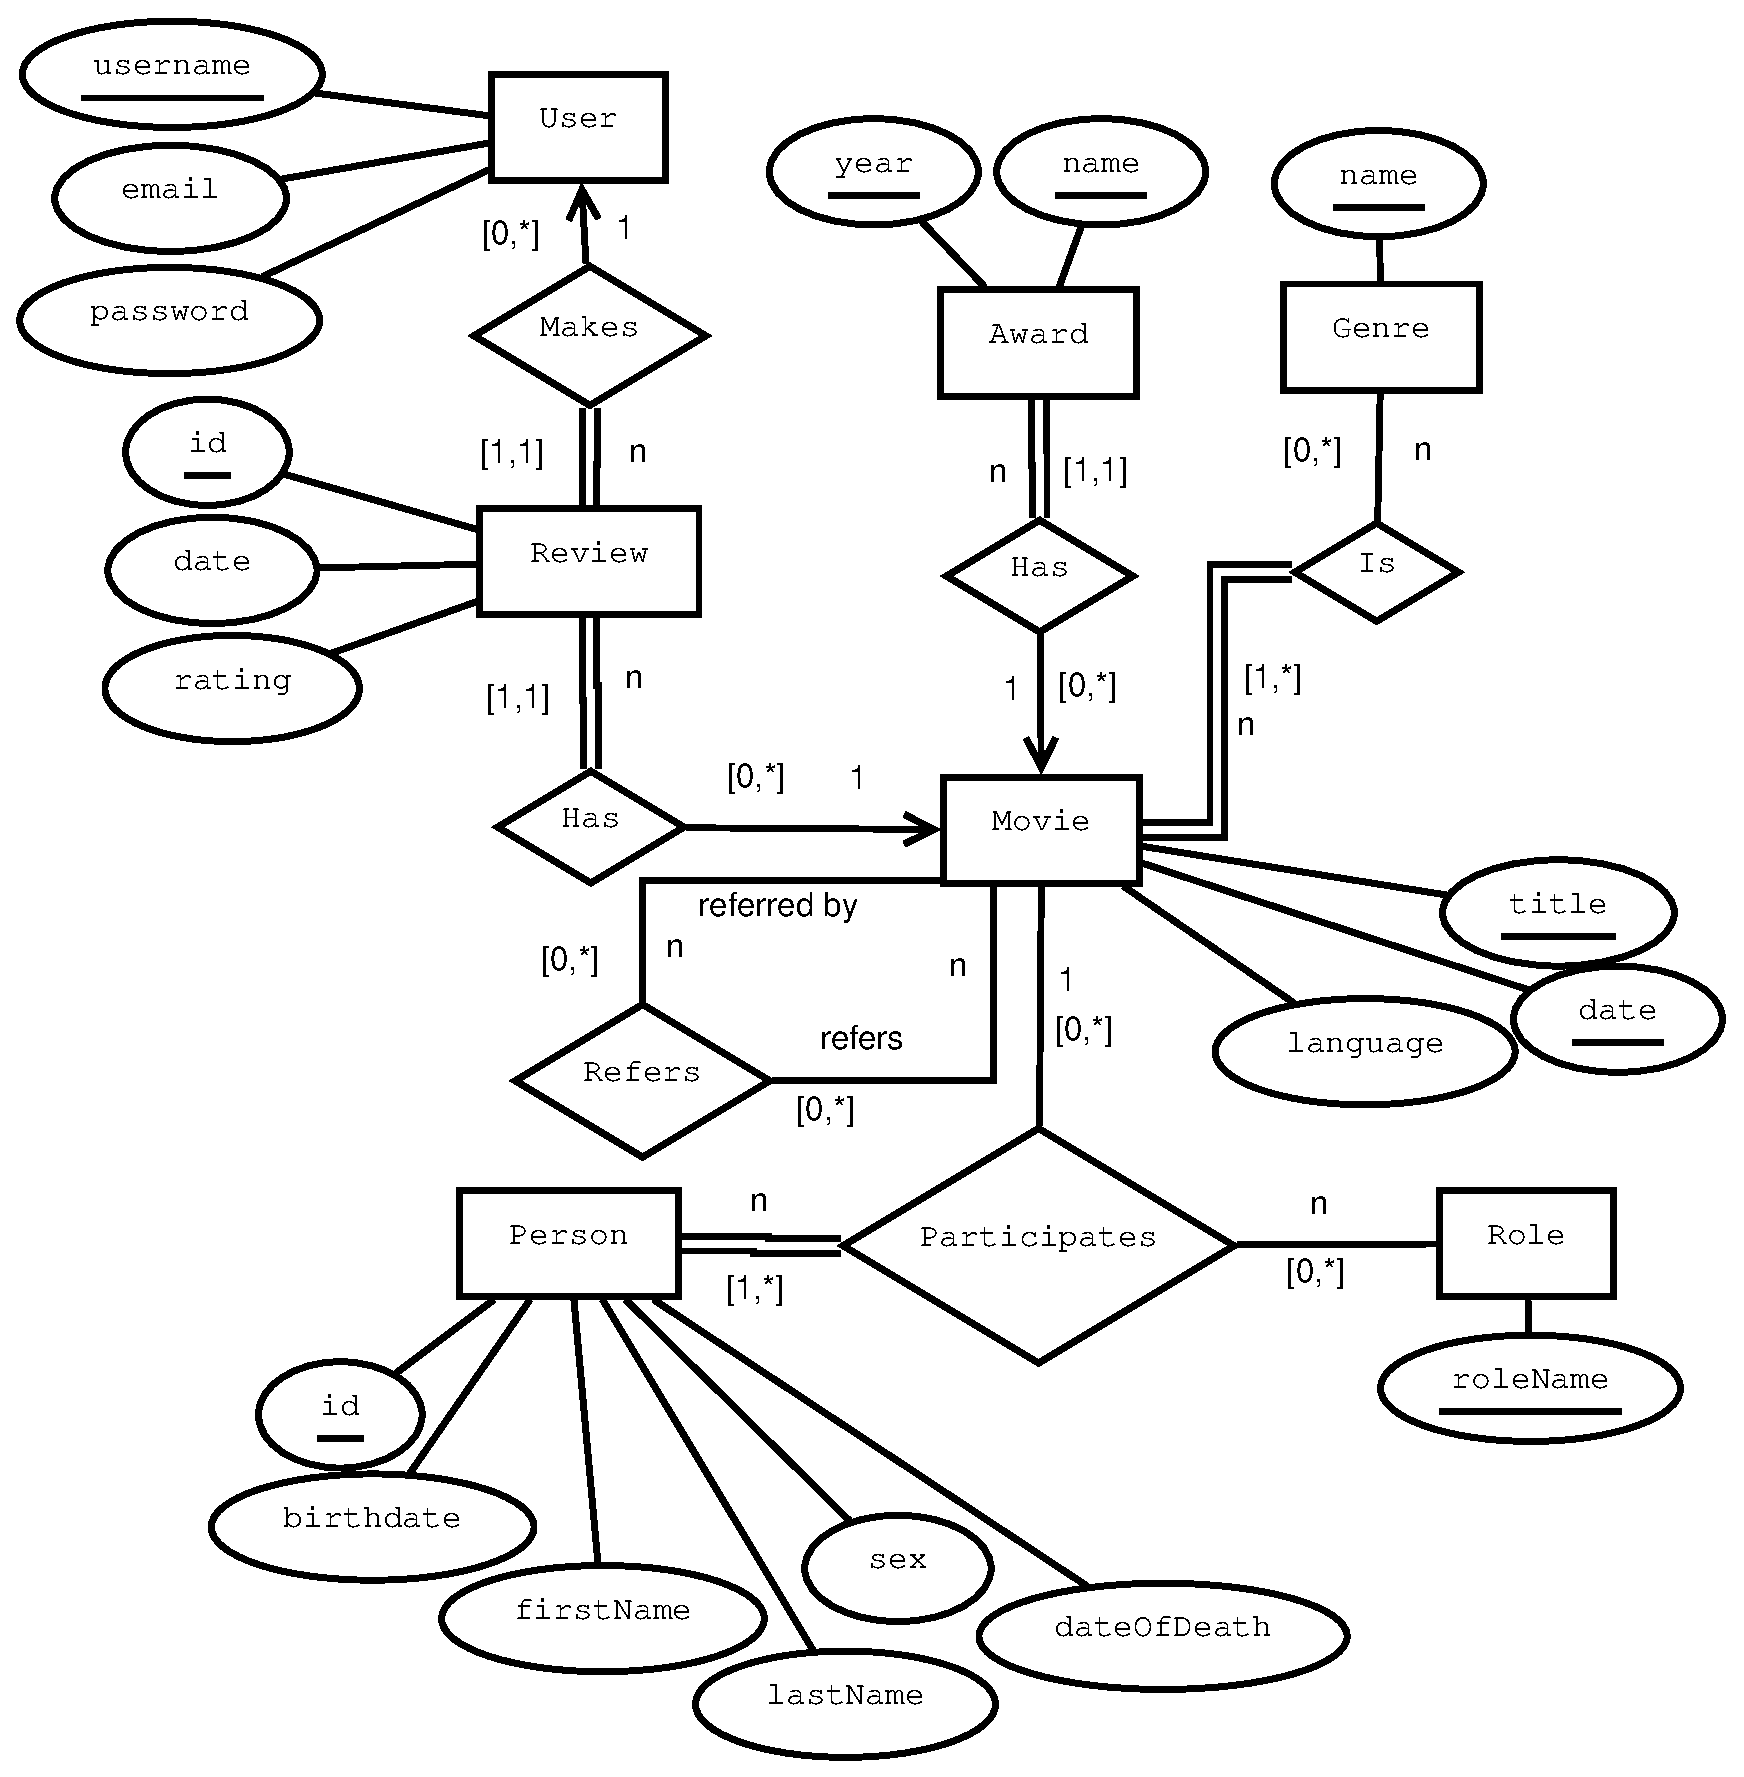
\includegraphics[width=\linewidth]{4-18.03.14/ERDiagram.eps}
  \caption{Revised ER diagram }\label{fig:ss4-er}
\end{figure}

\subsection{Functional dependencies}
\begin{itemize}
  \item User: username $\ra$ email, password
  \item Award: year, name $\ra$ title, date
  \item Movie: title, date $\ra$ language
  \item Person: id $\ra$ birthdate, firstName, lastName, dateOfDeath, sex
  \item Review: id $\ra$ rating, date, username, title, date
\end{itemize}

\subsection{List of normalized relations}

\subsubsection{Definitions}
This is also the derived relational schema. We simply derived thee following schema below by taking the mapped table and formalizing it. No algorithms were used.
\begin{itemize}
  \item User: \schema{\key{username : string}, email : string, password :string}
  \item Award: \schema{\key{year :integer, name : string}, \refs{title : string}{Movie}, \refs{date : string}{Movie}}
  \item Genre: \schema{\key{name : string}}
  \item GenreMovie: \schema{\key{\refs{name : string}{Genre}, \refs{title :string}{Movie}, \refs{date : date}{Movie}}}
  \item Movie: \schema{\key{title : string, date : date}, language}
  \item Refers: \schema{\key{\refs{title : string}{Movie}, \refs{date : date}{Movie}, \refs{referredTitle : string}{Movie}, \refs{referredDate : date}{Movie}}}
  \item Role: \schema{\key{roleName : string}}
  \item Participates: \schema{\key{\refs{title : string}{Movie}, \refs{date : date}{Movie}, \refs{roleName : string}{Role}, \refs{id : integer}{Person}}}
  \item Person: \schema{\key{id : integer}, birthdate : date, firstName : string, lastName : string, dateOfDeath : date, sex : string}
  \item Review: \schema{\key{id : integer}, rating : integer, date : date, \refs{username : string}{User}, \refs{title : string}{Movie}, \refs{date : date}{Movie}}
\end{itemize}

\subsubsection{Normalization}
We have not made any changes since all our relations are already on BCNF. It is obvious, that the relations with no functional dependencies are all on BCNF, that is: \textbf{Participates, Role, Refers, GenreMovie, Genre}.

For the remaining relations, User, Award, Movie, Person and Review, we say that they are all clearly on 1NF, since every attribute is atomic. For 2NF, every non-prime attribute must be fully functional dependent on each candidate key. For the User relation, every candidate key contains only a single attribute, and every non-prime attribute is thus fully functionally dependent on every candidate key. For the remaining relations, no subset of any candidate key exists such that a non-prime attribute is functionally dependent thereof. For 3NF, we need one of these 3 conditions to hold for each functional dependency $A \ra  B$:
\begin{enumerate}
  \item $A \ra B$ is trivial
  \item $A$ is a superkey
  \item $B$ is part of a candidate key
\end{enumerate}
For all functional dependencies $A \ra B$, we have that $A$ is a superkey, thus we conclude all our relations are on 3NF. For BCNF, all functional dependencies must meet one of the first two conditions just mentioned. Since they all meet condition 2, we now conclude that all of our relations are on BCNF.

\subsection{SQL for creating tables}
Below are SQL statements for creating each of the tables in our mapped relation.
\begin{lstlisting}[language=SQL]
CREATE TABLE user(
  username varchar(50),
  email varchar(50) UNIQUE NOT NULL,
  password varchar(50) NOT NULL,
  PRIMARY KEY(username)
);
\end{lstlisting}

\begin{lstlisting}[language=SQL]
CREATE TABLE award(
  year int,
  name varchar(50),
  title varchar(50) NOT NULL,
  date date NOT NULL,
  PRIMARY KEY(year, name)
);
\end{lstlisting}

\begin{lstlisting}[language=SQL]
CREATE TABLE genre(
  name varchar(50),
  PRIMARY KEY(name)
);
\end{lstlisting}

\begin{lstlisting}[language=SQL]
CREATE TABLE genreMovie(
  name varchar(50),
  title varchar(50),
  date date,
  PRIMARY KEY(name, title, date),
  FOREIGN KEY(name) REFERENCES genre(name),
  FOREIGN KEY(title, date) REFERENCES movie(title, date)
);
\end{lstlisting}

\begin{lstlisting}[language=SQL]
CREATE TABLE movie(
  title varchar(50),
  date date,
  language varchar(50),
  PRIMARY KEY(title, date),
);
\end{lstlisting}

\begin{lstlisting}[language=SQL]
CREATE TABLE refers(
  title varchar(50),
  date date,
  referredTitle varchar(50),
  referredDate date,
  PRIMARY KEY(title, date, referredTitle, referredDate),
  FOREIGN KEY(title, date) REFERENCES movie(title, date),
  FOREIGN KEY(referredTtitle, referredDate) REFERENCES movie(title, date)
);
\end{lstlisting}

\begin{lstlisting}[language=SQL]
CREATE TABLE role(
  roleName varchar(50),
  PRIMARY KEY(roleName)
);
\end{lstlisting}

\begin{lstlisting}[language=SQL]
CREATE TABLE participates(
  title varchar(50),
  date date,
  roleName varchar(50),
  id int,
  PRIMARY KEY(title, date, roleName, id),
  FOREIGN KEY(title, date) REFERENCES movie(title, date),
  FOREIGN KEY(roleName) REFERENCES role(roleName),
  FOREIGN KEY(id) REFERENCES person(id)
);
\end{lstlisting}

\begin{lstlisting}[language=SQL]
CREATE TABLE person(
  id int,
  birthdate date NOT NULL,
  firstName varchar(50) NOT NULL,
  lastName varchar(50) NOT NULL,
  dateOfDeath date NOT NULL,
  sex char(1) NOT NULL,
  PRIMARY KEY(id)
);
\end{lstlisting}

\begin{lstlisting}[language=SQL]
CREATE TABLE review(
  id int,
  rating int,
  dateOfReview date NOT NULL,
  username varchar(50) NOT NULL,
  title varchar(50) NOT NULL,
  date date NOT NULL,
  PRIMARY KEY(id),
  FOREIGN KEY(username) REFERENCES user(username),
  FOREIGN KEY(title, date) REFERENCES movie(title, date)
);
\end{lstlisting}

\subsection{Reflections}
After having completed self study 4, we can conclude that overall we believe we have a strong schema and grasp of creating tables that reduce redundancy and have the tools and skills to prove this.

After having learned the correct, standard notation, we can now pass this on to another developer to implement the database we have designed.

\subsubsection{Differences}
In self study 2, we fixed the relationships to reduce dependencies and express the fact that one actor (participant) can have multiple roles in a single movie.
